\subsection{Etap Release}
Faza wydania (\textit{Release}) koncentruje się na bezpiecznym przechowywaniu artefaktów oraz ich wersji, gotowych do wdrożenia w~środowiskach docelowych.

\subsubsection{Rejestr obrazów: Docker Hub}
Jako centralne repozytorium obrazów kontenerowych wykorzystano platformę \textbf{Docker Hub}.
\begin{itemize}
    \item \textbf{Rola w~projekcie:} Po pomyślnym zakończeniu etapu budowania i~testowania, obrazy mikroserwisów są wysyłane (ang. \textit{push}) do prywatnych lub publicznych repozytoriów w~Docker Hub. Każdy obraz jest oznaczony unikalnym tagiem (np. skrótem \textit{commit SHA} lub numerem wersji semantycznej), co zapewnia pełną identyfikowalność.
    \item \textbf{Uzasadnienie:} Docker Hub jest natywnie obsługiwany przez większość narzędzi CI/CD oraz klastry Kubernetes, co upraszcza proces pobierania obrazów podczas wdrożenia.
\end{itemize}

\subsubsection{Pakietowanie dla Kubernetes: Helm}
Zarządzanie manifestami YAML dla wielu mikroserwisów staje się trudne bez odpowiedniego narzędzia. Zgodnie z~decyzją \textit{ADR-0012}, jako standard pakietowania dla Kubernetes wybrano \textbf{Helm} — menedżer pakietów pozwalający na szablonowanie i~wersjonowanie konfiguracji infrastruktury.

\begin{techcard}{Helm}

\textbf{Opis:} Helm to menedżer pakietów dla Kubernetes, analogiczny do \texttt{apt} czy \texttt{brew} w~świecie systemów operacyjnych. Pozwala na definiowanie, instalowanie i~aktualizowanie złożonych aplikacji Kubernetes jako pojedynczych, wersjonowanych pakietów zwanych \textbf{chartami}. Chart to zestaw szablonów YAML sparametryzowanych wartościami z~pliku \texttt{values.yaml}. Helm śledzi historię wdrożeń jako kolejne rewizje, co umożliwia natychmiastowy rollback.

\textbf{Dobre nawyki:}
\begin{itemize}
  \item \textbf{Umbrella chart:} Grupowanie powiązanych mikroserwisów w~jeden chart pozwala wdrożyć cały stos jednym poleceniem \texttt{helm install}, zachowując spójność wersji wszystkich komponentów.
  \item \textbf{Parametryzacja przez values:} Wartości specyficzne dla środowiska (tagi obrazów, liczba replik, limity zasobów) powinny być wydzielone do osobnych plików \texttt{values-prod.yaml}, a~nie zakodowane na sztywno w~szablonach.
  \item \textbf{Wersjonowanie wydań (ang. \textit{releases}):} Każda zmiana wprowadzona przez \texttt{helm upgrade} tworzy nową rewizję. Polecenie \texttt{helm rollback} natychmiast przywraca poprzedni stan klastra bez ręcznej edycji manifestów.
  \item \textbf{Helpery szablonów (\texttt{\_helpers.tpl}):} Wspólne etykiety i~selektory należy definiować jako nazwane szablony w~\texttt{\_helpers.tpl}, aby zapewnić spójność i~uniknąć powielania kodu YAML.
\end{itemize}

\textbf{Rola w~projekcie:} Helm pełni rolę menedżera infrastruktury projektu. Umbrella chart \texttt{bsc-devops} opisuje wszystkie komponenty stosu w~jednym, wersjonowanym pakiecie.

\end{techcard}

\textbf{Umbrella chart i~parametryzacja środowisk:}
W~projekcie zastosowano wzorzec \textbf{umbrella chart}: jeden chart \texttt{bsc-devops} obejmuje wszystkie sześć komponentów stosu (serwisy \textit{users}, \textit{tasks}, \textit{task-archiver}, \textit{frontend}, bazę PostgreSQL oraz broker Pulsar). Każdy komponent może być niezależnie włączony lub wyłączony flagą \texttt{enabled}. Konfiguracja zasobów obliczeniowych i~tagów obrazów jest wydzielona do \texttt{values.yaml}:

\begin{lstlisting}[language=yaml, caption={Fragment \texttt{values.yaml} umbrella chartu --- parametryzacja serwisu \textit{users} (infrastructure/helm/bsc-devops/values.yaml)}, label={lst:helm-values}]
users:
  enabled: true
  image:
    repository: "docker.io/mateuszwas/users"
    tag: "1.2.0"
  replicas: 1
  resources:
    requests:
      cpu: "50m"
      memory: "64Mi"
    limits:
      cpu: "500m"
      memory: "256Mi"
\end{lstlisting}

\textbf{Szablony Go i~helpery:}
Szablony Helm korzystają z~silnika Go \texttt{text/template}. Wyrażenia \texttt{\{\{ include \}\}} wywołują nazwane helpery zdefiniowane w~pliku \texttt{\_helpers.tpl}. Przykładowo, helper \texttt{bsc-devops.imageRef} scala repozytorium z~tagiem obrazu, a~globalny tag może nadpisywać wartość per-serwis:

\begin{lstlisting}[language=yaml, caption={Fragment szablonu Deployment serwisu \textit{users} z~interpolacją wartości (infrastructure/helm/bsc-devops/templates/users.yaml)}, label={lst:helm-template}]
spec:
  replicas: {{ .Values.users.replicas }}
  template:
    spec:
      containers:
        - name: users
          image: {{ include "bsc-devops.imageRef"
            (dict "repo" .Values.users.image.repository
                  "tag"  .Values.users.image.tag
                  "ctx"  .) }}
          resources:
            {{- toYaml .Values.users.resources | nindent 12 }}
          livenessProbe:
            tcpSocket:
              port: 8080
            initialDelaySeconds: 10
            periodSeconds: 20
\end{lstlisting}

\subsubsection{Dystrybucja chartu: GitHub Container Registry}
Gotowy chart Helm jest publikowany jako artefakt OCI w~rejestrze \textbf{GitHub Container Registry} (GHCR). Dzięki natywnej obsłudze formatu OCI w~Helm 3.8+ możliwe jest traktowanie rejestru kontenerów jako uniwersalnego magazynu artefaktów --- bez potrzeby utrzymywania zewnętrznych repozytoriów chartów (np. ChartMuseum).

\textbf{Uzasadnienie wyboru GHCR:}
\begin{itemize}
    \item \textbf{Brak zewnętrznych zależności:} GHCR jest integralną częścią GitHub --- nie wymaga dodatkowych usług ani konfiguracji.
    \item \textbf{Jednolite logowanie:} Uwierzytelnianie odbywa się przez \texttt{GITHUB\_TOKEN} z~uprawnieniem \texttt{packages:write}, ten sam mechanizm co w~przypadku obrazów Docker.
    \item \textbf{Wersjonowanie OCI:} Tag artefaktu odpowiada wersji semantycznej chartu z~\texttt{Chart.yaml}, co zapewnia pełną identyfikowalność.
\end{itemize}

\textbf{Dwuetapowy proces publikacji:}
Dystrybucja chartu realizowana jest przez dwa oddzielne procesy CI/CD, powiązane zdarzeniem utworzenia tagu git. Podejście to rozdziela walidację od publikacji:

\begin{lstlisting}[language=yaml, caption={Proces CD publikujący chart do GHCR (.github/workflows/cd-helm.yml)}, label={lst:cd-helm}]
on:
  push:
    tags:
      - 'chart-apps-*'

jobs:
  publish:
    permissions:
      contents: read
      packages: write
    steps:
      - uses: actions/checkout@v7
      - uses: azure/setup-helm@v5
      - name: Log in to GHCR
        run: |
          echo "${{ secrets.GITHUB_TOKEN }}" | helm registry login ghcr.io \
            --username ${{ github.actor }} --password-stdin
      - name: Package chart
        run: helm package infrastructure/helm/bsc-devops
      - name: Push chart to GHCR
        run: helm push bsc-devops-apps-*.tgz oci://ghcr.io/${{ github.repository_owner }}/charts
\end{lstlisting}

Proces \texttt{ci-helm} waliduje chart i~--- przy każdym wypchnięciu zmian na gałąź \texttt{main} --- odczytuje wersję z~\texttt{Chart.yaml} i~tworzy tag git \texttt{chart-apps-<wersja>}. Tag ten wyzwala proces \texttt{cd-helm}, który pakuje chart poleceniem \texttt{helm package} i~publikuje artefakt OCI pod adresem \texttt{ghcr.io/mwas-inz/charts/bsc-devops-apps:<wersja>}.

Cały proces --- od walidacji, przez zdarzenie tagu, po konsumpcję opublikowanego artefaktu przez ArgoCD --- przedstawia rysunek~\ref{fig:chart-release}. Warto zauważyć, że tag jest wypychany tokenem osobistym (PAT), a~nie domyślnym \texttt{GITHUB\_TOKEN}: zdarzenia utworzone domyślnym tokenem nie wyzwalają kolejnych procesów, co stanowi zabezpieczenie GitHub Actions przed nieskończonymi pętlami.

\begin{figure}[H]
    \centering
    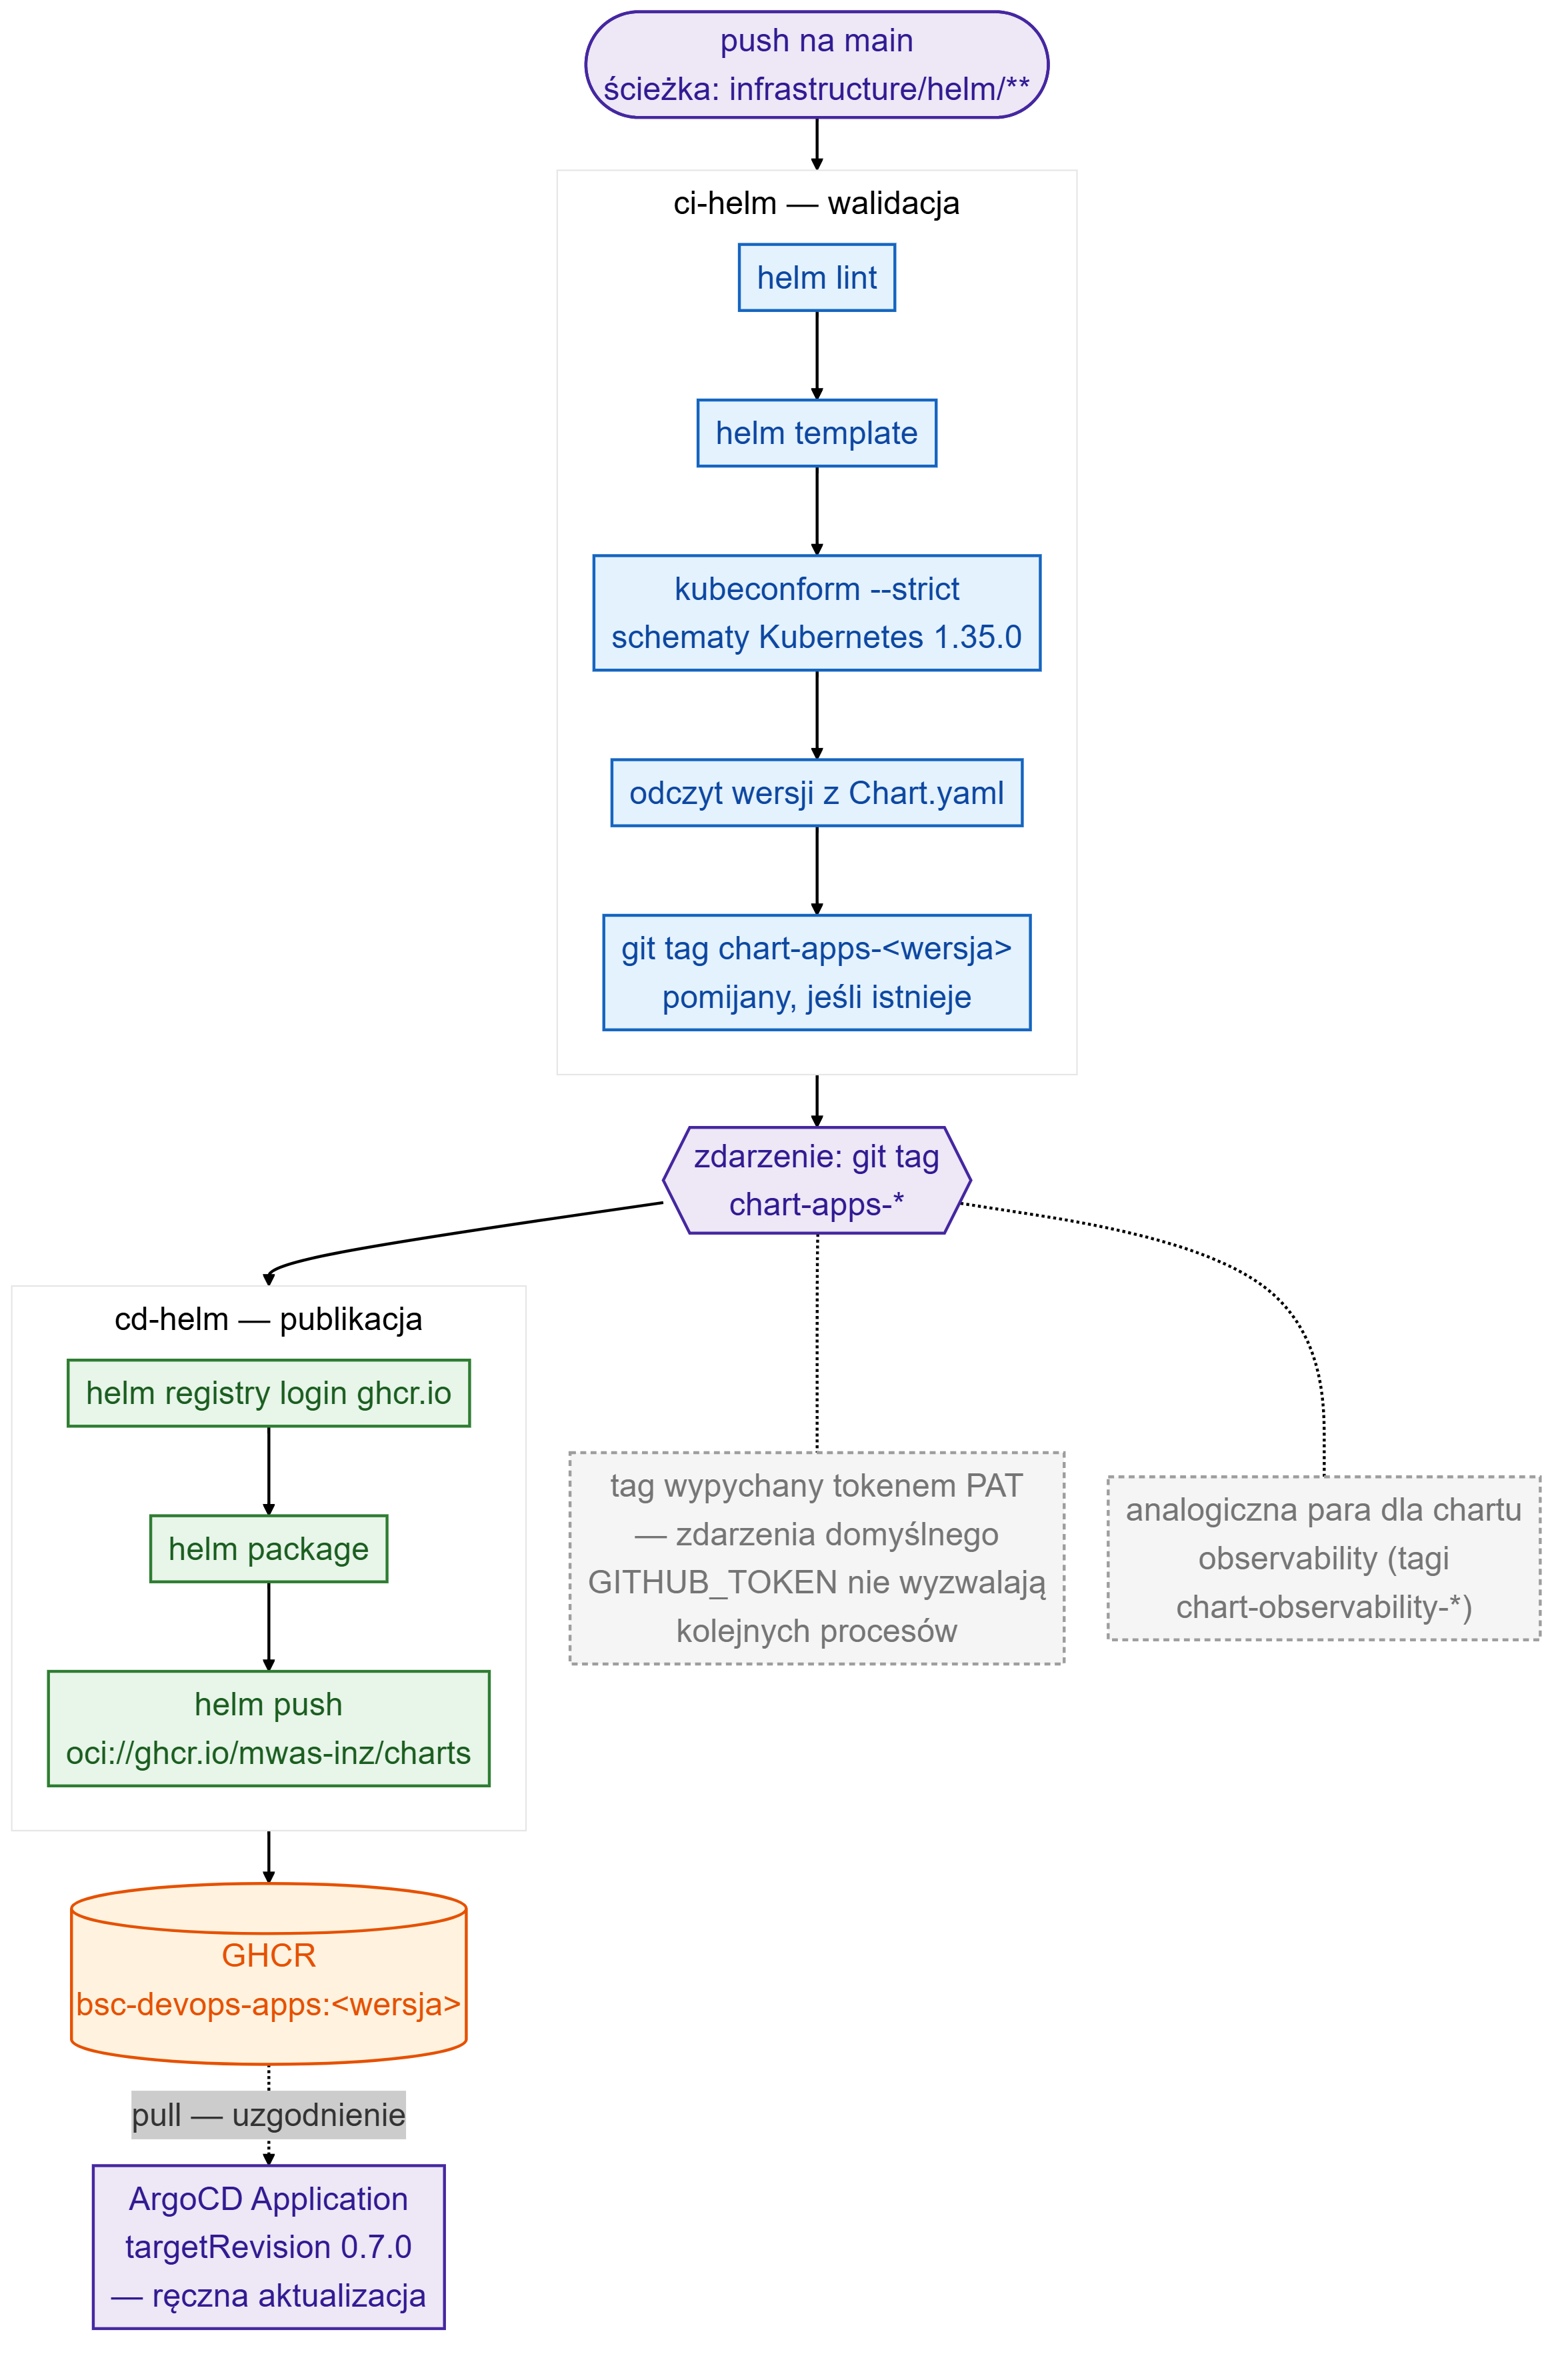
\includegraphics[width=\textwidth]{img/diagrams/06-release/release-01-flow-chart-release.png}
    \caption{Dwuetapowy proces publikacji chartu --- walidacja (\texttt{ci-helm}) oddzielona od publikacji (\texttt{cd-helm}) niezmiennym git tagiem \texttt{chart-apps-<wersja>}; artefakt OCI konsumowany przez ArgoCD według przypiętej wersji (opracowanie własne).}
    \label{fig:chart-release}
\end{figure}
